\documentclass[9pt,journal]{IEEEtran}

\ifCLASSOPTIONcompsoc
  % IEEE Computer Society needs nocompress option
  % requires cite.sty v4.0 or later (November 2003)
  \usepackage[nocompress]{cite}
\else
  % normal IEEE
  \usepackage{cite}
\fi

\usepackage{amsmath,amssymb,amsfonts}
\usepackage{algorithmic}
\usepackage{graphicx}
\usepackage{textcomp}
\usepackage{xcolor}

\hyphenation{op-tical net-works semi-conduc-tor}

\def\BibTeX{{\rm B\kern-.05em{\sc i\kern-.025em b}\kern-.08em
		T\kern-.1667em\lower.7ex\hbox{E}\kern-.125emX}}

\makeatletter
\def\endthebibliography{%
	\def\@noitemerr{\@latex@warning{Empty `thebibliography' environment}}%
	\endlist
}
\makeatother

\makeatletter
\newcommand*\titleheader[1]{\gdef\@titleheader{#1}}
\AtBeginDocument{%
	\let\st@red@title\@title
	\def\@title{%
		\bgroup\normalfont\large\centering\@titleheader\par\egroup
		\vskip1em\st@red@title}
}
\makeatother


\begin{document}
\bstctlcite{IEEEexample:BSTcontrol}

\title{Parallel Patterns with C and OpenMP}


\author{
	{
		Filipe~de Luna,~\IEEEmembership{48425} and
        Gabriel Batista,~\IEEEmembership{47590}
    } \\ Department of Informatics - FCT-NOVA
        
}

\markboth{Concurrency and Parallelism - DI FCT-UNL, 2019-2020}%
{Concurrency and Parallelism - DI FCT-UNL, 2019-2020}

% make the title area
\maketitle

\section{Introduction}
For the Concurrency and Parallelism course of the Integrated Masters in Computer Science at FCT-NOVA, we were asked to implement a series of parallel patterns using the \textit{OpenMP} API. The following document describes our implementation of these patterns, the results we’ve achieved during the testing phase and our interpretation of these same results.

\section{Tools Used}

We developed the project in \textit{Linux} using \textit{C} language and the \textit{GCC} compiler, writing our code in \textit{Clion} and using \textit{CMake} for building. We used the standard \textit{GNU} argument parser (argp) \cite{argp}, to make testing a lot easier by adding flags and arguments to our program such as: test id, debug mode, thread count and weight enabling.

Our most important tool was \textit{OpenMP} \cite{omp}, a multi-platform API that allows the user to add pragmas to programming blocks in order to parallelize code. The main perk of \textit{OpenMP} is that parallel code ends up looking extremely similar to serial code, meaning serial execution is still possible.

\section{Testing Methodology}

We have created two python scripts to aid us in testing.

The first script, named “tester”, runs the program several times with the appropriate flags and saves the results. The tester can be configured to run a specific algorithm or all with a set of numbers of jobs, number of threads and, lastly, the number of repetitions for every test/number of jobs/thread combo. From these repetitions, we extract a mean value for a more accurate result. All these results are written to a file of our choosing.

The tester also allowed for configuring tests to run with different sets of numbers of jobs, since some algorithms run a lot faster than others and we needed to keep overall testing times low.  Another parameter, was “weight”, which activated a flag in the program that added a for loop with a configurable number of iterations for every worker. Ideally, we would increase the number of total jobs, but this wasn't really viable as the worker was really light and for the number of needed jobs, it would result in running out of RAM. This was necessary since some algorithms had a very significant management cost and it allowed us to simulate a heavier work load in order to visualize their gains more accurately. 

The second python script, the “grapher”, reads the output file with the results and creates a graph for each test, using \textit{Matplotlib} \cite{matplotlib}, in order to help us visualize the data. 

Since our computers had a limited core count, we couldn’t get a realistic perception of the gains that the parallelization of these patterns could allow for. So we ran our tests in the cluster maintained by our Faculty’s Department of Informatics. The particular node we used for tests had 64 cores.

For profiling we ran the \textit{CLion} default profiler (\textit{perf} on our Linux systems) on a machine with 16 threads (8 physical + 8 logical). Profiling was incredibly useful to get an idea of how much the management cost was, and how much time was spent doing serial work.

After inspecting the profiler results in the 16 thread CPU, we noticed that the added weight resulted in a very significant reduction of the percentage of time spent in creating the threads. So we decided to run all tests with an added weight of 250 for iterations on the cluster.

To get realistic results for each thread count, we disabled \textit{OpenMP's} default dynamic scheduling and forced it to static. This means that the number of threads we specified will actually be used, instead of \textit{OpenMP} dynamically optimizing the thread count for the given workload. Even though this might result in worse results and isn't suitable for a real live application, it is ideal to obtain the accurate results we need for our tests.

\section{Mandatory Parallel Patterns}

% Map --------------------------------------------------------------	
\subsection{The Map Pattern}
\label{map}

\subsubsection{Implementation}

The Map pattern was the simplest and most straightforward to implement since we can use \textit{OpenMP's} for construct to map $ n $ jobs to a for loop with n iterations. This for loop will then be proportionally sliced with each thread receiving a similar slice. Since there are no dependencies between jobs or a necessary order of execution, this algorithm becomes embarrassingly parallelizeable \cite{mccool}.

\subsubsection{Testing}

With 10.000 jobs, the algorithm showed a linear speedup up to 4 cores, with the speedup severely lowering when 8 were used. With upwards of 8 cores, we saw similarly linear negative speedup, since the management cost for the creation of these threads was more than the time the threads actually ran their work. Only at 500.000 jobs did the algorithm start showing the expected linear speedup by increasing threads up to the physical core count of the machine.

With an added weight of 1000 for iterations and 16 threads on 10.000.000 jobs, it's possible to observe, in the profiler, that the program spends ~93\% of the time running in parallel. By removing the added weight, we end up with ~68\% of time running in parallel. It's easy to conclude that the necessary workload per job for the pattern to become viable is not that big, as a for with 1000 iterations is an extremely fast computation in a modern chip.

% Reduce --------------------------------------------------------------		
\subsection{The Reduce Pattern}
\label{reduce}

\subsubsection{Implementation}

Although \textit{OpenMP} includes a reduction construct and can efficiently parallelize reductions, this only works for scalar values and arithmetic operations \cite{ompreduct}. Since we want to create a generic reduction, allowing for any type of values, we had to implement a custom reduction algorithm. The algorithm was based on the one found McCool's book, using a 2-phase reduction \cite{mccool}. In the first phase, each thread gets a similar portion of the total work and reduces it (much like a map), and in the second phase, those results are reduced serially. 

\subsubsection{Testing}

As expected, this algorithm showed results very similar to the ones from the map, as it behaved very similarly to one. Since the second phase only has a maximum of jobs equal to the number of threads, it does not scale significantly and shouldn't affect the gains much, even though it is executed serially.

Since the computational weight of the serial computation is not significant, as mentioned earlier, the profiling showed similar results to map (\ref{map}).

% Scan --------------------------------------------------------------		
\subsection{The Scan Pattern}
\label{scan}

\subsubsection{Implementation}

The scan pattern was the most complicated to implement of all the mandatory algorithms. There were many possibilities but we eventually decided on the inclusive three-phase algorithm shown on McCool's book on chapter 5.5 \cite{mccool}. The first two-phases are almost identical to the reduce pattern mentioned earlier in reduce (\ref{reduce}), with the third one using their result of the first value of each slice to compute the following values. Like in reduce, the second phase is serial and has as many computations as the amount of threads executing the algorithm. 

An exclusive scan was created which was just a call to this function which basically does an inclusive scan with an offset of 1, so the first value is 0.

\subsubsection{Testing}

The scan did not show improvements from switching from 1 to 2 threads in every number of jobs, with the added management costs being higher than the gains up to 1.000.000 jobs (the maximum we've tested). But from upward of 2 threads, the gains were linear up to 32 threads, with very small improvement from 32 to 64 threads. 

The reason behind the performance being equal or worse with two threads is due to the fact that this implementation uses $ n - 1 $ threads for the first cycle and the second cycle is serial. This means that, with 2 threads, 2 out of 3 phases are executed serially, with the added management cost not making it worth the extra parallelism in the last phase.

Again, similarly to reduce (\ref{reduce}), the profiling showed similar results to map (\ref{map}). With the expected parallelism with 2 threads, as mentioned in the last paragraph, resulting in only ~33\%. We conclude this algorithm is not a good solution for very low thread counts.

The scan was actually one of the algorithms that ended up showing better results with a higher thread count than the physical cores on the machine. This a phenomenon McCool describes as "Parallel Slack" \cite{mccool}, which ends up giving more flexibility to \textit{OpenMP}, as it can better distribute these chunks of jobs per threads as it sees fit. If there were a many chunks as threads, one hanging thread would hang the entire program.

% Pack -------------------------------------------------------------	
\subsection{The Pack Pattern}
\subsubsection{Implementation}
\label{pack}

Even though we studied McCool's pack chapters from the book, most of our ideas for pack came from his article on \textit{Dr. Dobb's} on pack \cite{dobbpack}. The main idea is that pack is not a fundamental pattern, meaning it can be implemented by combining others. 

We chose to do an exclusive scan on the filter so that the resulting array would give us the correct position in the destiny array for each item of the source array that is allowed in the filter. We then run a map on the source array, and for each position we check if it is allowed in the filter and, if so, we send it to the position given by the scanned filter array.

\subsubsection{Testing}

To test pack, we created a filter array with the same size as the number of jobs. This array had alternating ones and zeros.

The pack results seem, at first, really odd as it gets worse performance as the core count grows up to around 500.000 jobs. And, even between 500.000 and 1.000.000 jobs, it shows a linear speed up from 2 to 8 cores and then it starts showing a linear negative speedup.

On closer inspection, we notice that pack does not use a worker, but a \textit{memcpy} instruction that is only executed $ n / 2 $ times, with $ n $ being the number of jobs. This means that not only is this job not affected by the weight, but also has a lot lighter computations. Even though it uses a scan, the worker used for the scan is custom and does not include weight.

This results in a lot faster computation, making the algorithm finish much faster than the others for the same number of jobs. And, this also means that even though it shows a good parallelization percentage with upwards of 80\% in the profiler, it does not spend enough time running to make up for the management cost of a high number of threads. Since it becomes impossible to increase the number of iterations due to RAM limitations, we can only "guess" that it would need a more demanding workload of 10.000.000+ jobs to start showing a linear speedup up to the number of threads of cluster.

% Gather --------------------------------------------------------------	
\subsection{The Gather Pattern}
\label{gather}

\subsubsection{Implementation}

Gather's implementation was very similar to pack's (\ref{pack}), with a \textit{memcpy} instruction and a map. The gather was based on the idea's in \textit{Dr. Dobb's} that a gather is parallel read of elements of memory that subsequently writes said values to another array according to a filter. This filter holds the position in the source array of the element to write for each position, with each index $ i $ of the filter mapping to the same index $ i $ of the destiny array.

\subsubsection{Testing}

For testing, we created a filter with the same size as there were jobs and populated it with random integers that could be anywhere between 0 and $ n - 1 $, with n being the number of jobs.

Since the implementation is very similar to pack's (\ref{pack}), the results were basically the same. Gather does execute a \textit{memcpy} always instead of pack's conditional, but the amount of jobs (or job size) necessary to see a difference from this verification is immense as \textit{memcpy} is incredibly fast for byte-sized copies.

% Scatter --------------------------------------------------------------	
\subsection{The Scatter Pattern}
\label{scatter}

\subsubsection{Implementation}

Our default implementation of scatter is the atomic scatter which is briefly mentioned in McCool's book, making us have to come up with our own solution. We found this variation of scatter particularly hard to implement due to not being able to use \textit{OpenMP's} \textit{atomic} pragma, as it does not work with \textit{memcpy}. Since \textit{memcpy} writes data block by block, two parallel writes can cause a corruption as the destiny can have part of the information from the first job and part from the second.

Our solution was to use a custom quicksort that ordered the filter and the reordering of positions was reflected on the source array. By doing so, it was possible to add a conditional \textit{critical} pragma when the next value in the filter is equal to the current. This results in a very heavy reduction of the use of the \textit{critical} pragma and a good parallel performance at the cost of the initial quicksort computation.

\subsubsection{Testing}

The added quicksort at the beginning turned this algorithm from $ O(n) $ into $ O(n\log_n) $, meaning the computation needed to be really intense in the parallel phase to make up for the added quicksort computation. 

In our tests we made it possible to set the size of the destiny array. The probability of triggering a critical section is $ 1 / n $, with $ n $ being the number of destiny positions. But this does not mean $ 1 - 1 / n $ of the original speed, because the \textit{critical} section halts all the threads. 

With a low destiny array of just 10 positions, we only managed a parallelization of around 5\% because we kept hitting the \textit{critical} section. After changing the destiny array size to $ n / 50 $, with $ n $ being the number of jobs, the profiler showed around 80\% parallelization time, due to hitting the \textit{critical} section much less.

Since running with only 10 positions in the destiny array resulted in so many collisions, we also had to run a lower number of jobs and the resulting speedups weren't satisfactory as it only showed a significant speedup starting at 50.000 iterations and only up to 8 threads. After 8 threads, the effects of the \textit{critical} section overcame the added parallelization. With $ n / 50 $ positions in the destiny array, the algorithm ran a lot faster, but the speedup was relatively similar. 

During testing, we concluded the reason for showing worse results with additional threads is due the \textit{critical} section halting more work and being a lot more complex as there are more threads to manage. This is also called "lock management overhead", which increases with the number of threads \cite{lockmanage}. Therefore, this algorithm does work, but does not scale well, at all and its performance is completely tied to the size of the destiny array.

% Pipeline --------------------------------------------------------------	
\subsection{The Pipeline Pattern}
\subsubsection{Implementation}

The pipeline is an algorithm that does a collection of operations on a collection of data in order. The default pipeline implementation we chose was the map pipeline briefly discussed on McCool's book \cite{mccool}. This algorithm is just a succession of maps, with each map traversing all the data and executing the respective operation.

\subsubsection{Testing}

Since this algorithm relies on maps, which are embarrassingly parallel, it comes as no surprise that the profiler confirms this, with over 80\% of the time running in parallel.

For testing, a group of three workers were chosen that: multiplied the value by two, incremented and then divided the result by two.

The speedup was also pretty linear until the number of physical threads was reached, showing a little more improvement with 128 threads due to the parallel slack phenomenon mentioned earlier in scan (\ref{scan}). However, the algorithm only started showing consistent results starting with 100.000 iterations, meaning that this is when the management cost stops affecting the gains obtained from parallelizing.

% Farm --------------------------------------------------------------	
\subsection{The Farm Pattern}
\subsubsection{Implementation}

The farm pattern is very hard or next to impossible to implement in \textit{OpenMP}, since we can't have a fine-grained control of threads. \textit{OpenMP} dynamically distributes and hands work to threads. We can ask \textit{OpenMP} to use $ n $ threads in a computation, but we can't choose which threads will be used, and controlling them is hard.

\textit{OpenMP} contains a \textit{task} pragma that is an implementation of a farm pattern \cite{jlfarm}. With \textit{task} we can add computational tasks to a queue from which \textit{OpenMP} will dynamically distribute throughout all the threads however it sees fit.

This is the implementation we went for. For each job we create a \textit{task} and \textit{OpenMP} distributes it through the number of threads we set. The loop that creates all the \textit{tasks} needs to be executed by a single thread who acts as a master, and afterwards it will also become a slave, joining all the other threads in consuming \textit{tasks}.

\subsubsection{Testing}

With an added weight of 250 iterations in every worker, we saw a linear negative speedup as we increased the number of threads, throughout all the numbers of iterations. When the weight was increased to 15.000 iterations, we could observe a linear speedup up to 16 cores. With upwards of 16 cores, the speedup would exponentially negatively grow, with 64 threads taking more time than a single one. But, in the case of 128 threads, it lowers the time exponentially and is almost at its fastest.

After some investigation, we've traced the culprit of this odd phenomenon - \textit{OpenMP} itself - as it increases the time to create a \textit{task} as more threads are used \cite{granularity}. Another interesting feature is "\textit{task} throttling", an internal mechanism in \textit{OpenMP} that forces \textit{task} serialization after a specific number of \textit{tasks} have been created \cite{granularity}. As to why using 128 threads results in an incredible speedup, we believe it is attributed to the fact that, besides of the expected parallel slack, increasing the number of threads also increases the maximum number of \textit{tasks} before it begins \textit{task} throttling.

Since this implementation has little to no significant serial work, we can expect it to be embarrassingly parallel. We confirm this when we run the profiler and consistently upwards of 90\% of the time in parallel work.

We can conclude that \textit{OpenMP} isn't suited to implement farm and that tasks come with a heavy management cost. 

\section{Extra Parallel Patterns}

% Priority Scatter --------------------------------------------------------------	
\subsection{The Priority Scatter Pattern}
\subsubsection{Implementation}

In this version of scatter, the order of the job in the array dictates its priority. This pattern is briefly discussed in the book \cite{mccool}. This pattern does not take into account collisions as subsequent writes will overwrite previous data and yield a deterministic result based on the order.

The implementation of this pattern was pretty straightforward as it's essentially an \textit{OpenMP} \textit{for} construct with an \textit{ordered} construct, forcing it to execute the iterations in order \cite{omporder}.

\subsubsection{Testing}

This pattern shows consistently worse performance for all numbers of jobs as the number of threads increases, up to 1.000.000 iterations. We can attribute this to the fact that it shares the same issue as gather \ref{gather}, as it behaves similarly. This issue, is the fact that \textit{memcpy} is too fast and the number of jobs needed to make up for the management cost of the added threads is enormous.

As expected, if we add a for loop with 1000 iterations the management cost stops being relevant and we get a continuous linear speedup up to the number of physical cores. 

% Item-Bound Pipeline --------------------------------------------------------------	
\subsection{The Item-Bound Pipeline Pattern}
\label{itembound}

\subsubsection{Implementation}

This implementation of the pipeline was based on slides explaining the pipeline pattern from the University of Oregon \cite{pipelineoregon}. It's item-bound nature basically means a thread takes a job and executes all the workers at once on it, taking advantage of data locality.

The implementation is pretty straightforward as it is basically an \textit{OpenMP} \textit{for} construct that at each job, executes all the workers.

\subsubsection{Testing}

As expected, this algorithm is embarrassingly parallel, with the profiler reporting around over 90\% time spent in parallel computations and shows a linear speedup up to 32 threads and a smaller speedup up to 128, due to parallel slack.

% Serial Pipeline --------------------------------------------------------------	
\subsection{The Serial Pipeline Pattern}

\begin{figure}[htbp]
	\centerline{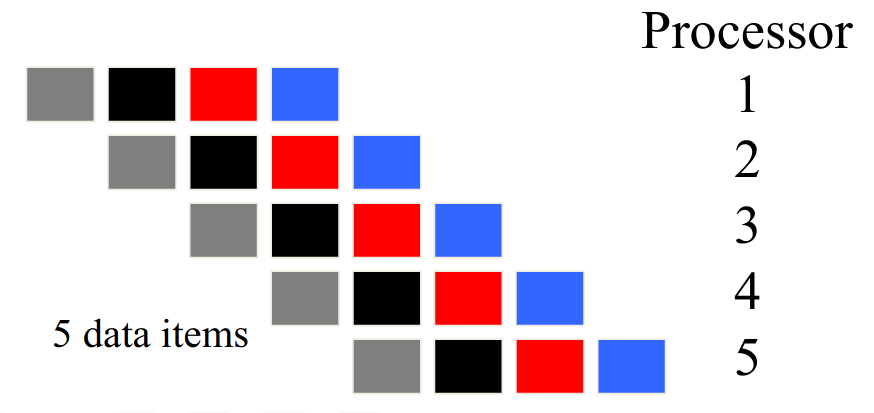
\includegraphics[scale=0.1]{img/serialpipeline.png}}
	\caption{ A serial pipeline. \cite{pipelineoregon} }
	\label{serialpipe}
\end{figure}

\subsubsection{Implementation}

Like the item-bound pipeline (\ref{itembound}), this implementation was based on slides  from the University of Oregon \cite{pipelineoregon}. The main purpose of this algorithm is to allow for various tasks (in this case a collection of workers that work on a single piece of data (job)) that cannot be parallelized, to run through a parallel pipeline. 

As we can see from figure \ref{serialpipe}, the serial pipeline starts executing a job after the last one has executed its first worker. This means that it for the first and last $ n - 1 $ cycles, with $ n $ being the number of workers, it won't be able to make full use of it's parallelization potential. 

Another problem with this pipeline is that it only makes sense to have as many threads as there are workers, and the number of workers limits the amount of threads it can make use of.

The implementation is basically a for loop with an \textit{OpenMP} \textit{for} construct inside. The outer for accounts for the amount of steps the total algorithm takes from the first job's first worker to the last job's last worker. The inner \textit{for} construct does runs the expected worker in each data for this step.

\subsubsection{Testing}

For testing, the number of workers were set to 64 (the maximum number of physical threads on the machine). Since the number of jobs is considerably larger than the number of workers, the first and last $ n - 1 $ cycles, mentioned earlier, don't make much of a difference.

The large number of workers makes this algorithm take a lot of time since, not only is the amount of work multiplied by the amount of workers, but also each worker has the inherent weight. So, to combat this, the number of jobs executed was heavily lowered to a maximum of 10.000.

With the default weight of 250 iterations, there was an acceptable linear speedup up to 8 threads improvement starting at 500 jobs and up to 10.000.

After raising the weight of the workers to 10.000 iterations the tests showed the expected linear speedup all the way to the number of threads on the machine (64). It's possible to conclude the necessity for such a high weight in a job to make up for the management cost is because, since the \textit{OpenMP's} \textit{parallel} construct is inside a for loop, the management cost is multiplied by the iterations of that same for loop.

% Stencil --------------------------------------------------------------	
\subsection{The Stencil Pattern}

\subsubsection{Implementation}

The stencil implementation was based on the one that is demonstrated in chapter 7.1 of McCool's book \cite{mccool}. Stencil is similar to a map, but every job is computed from the result of the computation of itself and the $ n $ jobs in its vicinity. It's a technique that is used in image manipulation software, for instance, so that a pixel gets a color that is the average of the pixels around it.

The implementation was straightforward as it is essentially a map, but instead of just doing it's respective worker, it creates a temporary variable to hold the reduction from the value that is $ n $ positions behind it to the one that is $ n $ positions in front, with $ n $ being the size of the vicinity to take into account. After computing this reduction, it stores the value in its respective place of the destiny array.

\subsubsection{Testing}

For testing, we set the number of jobs in the vicinity to be computed to 5. This means that, unless we're at an edge, we reduce 11 jobs for each job, which results in a lot more computations for each job. To account for this, less total jobs were ran.

At 50.000 jobs, the cost of management was compensated for and it was possible to observe an almost linear speedup up to the number of physical threads in the machine (64).

Since this algorithm is a variation of a map, it's embarrassingly parallel and the profiler shows over 90\% of the time is spent in parallel computation.

% Parallel Prefix --------------------------------------------------------------	
\subsection{The Parallel Prefix Algorithm}

\subsubsection{Implementation}

\begin{figure}[htbp]
	\centerline{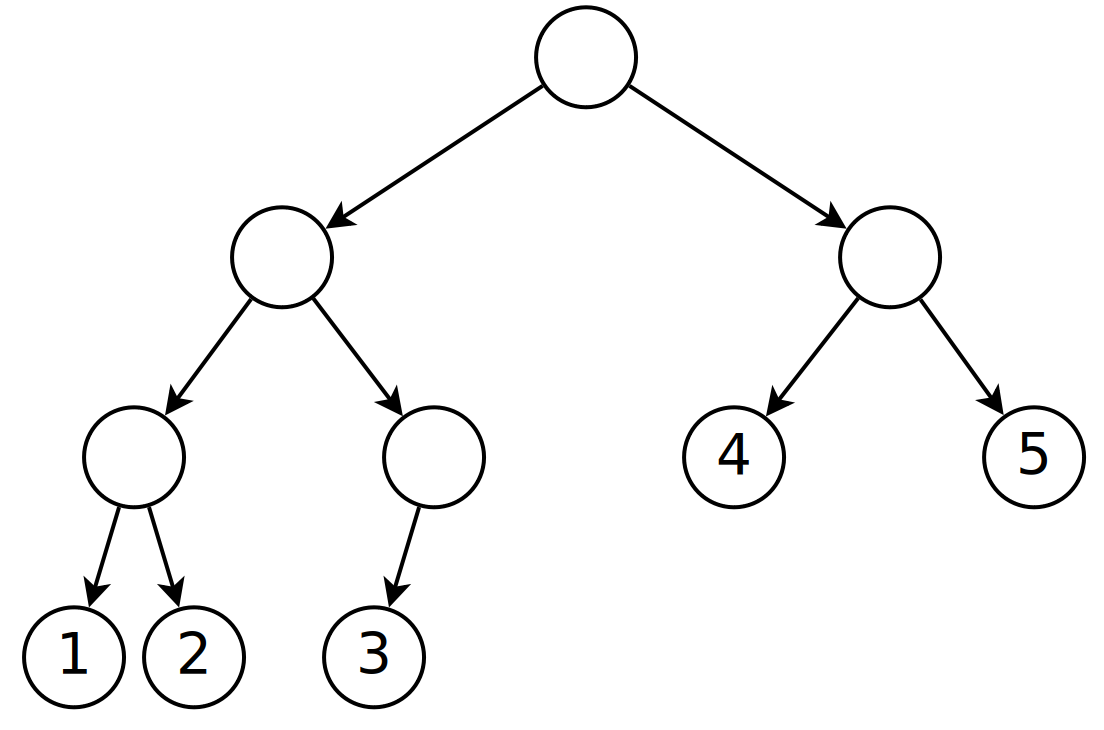
\includegraphics[scale=0.1]{img/parprefix.png}}
	\caption{ Parallel-Prefix without a power of 2. }
	\label{parprefix}
\end{figure}

The parallel-prefix is an algorithm that implements the scan pattern. Our implementation of the parallel-prefix algorithm was based on the slides by David Walker from Princeton University  \cite{parprefix}. This algorithm maps an array of jobs to the bottom of a tree and does two passes - one up pass and one down pass. The first pass computes the result of the computations bottom-up, while the second one traverses the tree top-down to compute the prefixes - which are basically the aggregated value from the node at the left. At the leafs, we can compute the result of the operation involving the sum (which is the respective value in the source array at this level) and the prefix, to get the aggregated value of the scan up until that position.

The parallel prefix was an extremely difficult algorithm to implement since we wished for it to be compatible with any number of jobs, not just powers of 2, as shown in figure \ref{parprefix}, where the we divide the number of jobs between the last two layers. 

Essentially, a tree will have either $ 2n - 1 $ or $ 2(n - 1) $ elements, where $ n $ is the number of jobs and the respective height will be $ \log_2(m) + 1 $ where $ m $ is the number of elements. Our implementation is basically succession of maps, with each one being respective to a level of the tree. At each node we make a few verifications like if, the node is at the last level or if it is a leaf and then we compute the sum or the prefix value, depending on the pass. 

\subsubsection{Testing}

Like many other algorithms before, the Parallel-Prefix becomes almost embarrassingly parallel when the number of jobs greatly exceeds the number of threads, since the computations at the upper levels stop being so significant. As expected, for 10.000 jobs, the profiler shows that around 90\% of the time, the algorithm is running in parallel.



\section{Acknowledgments}

\bibliographystyle{IEEEtran}
\bibliography{IEEEabrv,biblio}{}

\section{Work Division}

\section{Comments}


\end{document}


